\documentclass[11pt]{article}
\usepackage[margin=1in]{geometry}
\usepackage{amsmath,amssymb}
\usepackage{graphicx}
\usepackage{booktabs}
\usepackage{hyperref}
\usepackage{natbib}
\usepackage{doi}
\hypersetup{colorlinks=true,linkcolor=blue,citecolor=blue,urlcolor=blue}
\newcommand{\ScalingRows}{2 & 100.0 & -- & 123.2 & 2.00 \\
3 & 66.7 & 76.2 $\pm$ 0.1 & 76.2 & 3.00 \\
4 & 50.0 & 54.6 $\pm$ 0.4 & 54.9 & 4.00 \\
5 & 40.0 & 42.4 $\pm$ 0.4 & 42.8 & 5.00 \\
6 & 33.3 & 34.7 $\pm$ 0.3 & 35.1 & 6.00 \\
7 & 28.6 & 29.4 $\pm$ 0.1 & 29.7 & 7.00 \\
8 & 25.0 & 25.5 $\pm$ 0.0 & 25.8 & 8.00 \\
}
\newcommand{\ExcessMinMs}{0.5}
\newcommand{\ExcessMaxMs}{9.5}
\newcommand{\Nmax}{8}
\newcommand{\IntervalNeight}{25.5}
\newcommand{\PredNeight}{25.0}
\newcommand{\RateZero}{26.7}
\newcommand{\GammaStar}{13}
\newcommand{\TdecStarMs}{76}
\newcommand{\GapHagan}{760}
\newcommand{\GapTegmarkOrders}{12}
\newcommand{\DecoherenceRows}{0 & 26.7 & 5.77 \\
1e1 & 16.7 & 3.86 \\
3e1 & 3.3 & 1.05 \\
1e2 & 0.0 & 0.21 \\
3e2 & 0.0 & 0.07 \\
1e3 & 0.0 & 0.02 \\
3e3 & 0.0 & 0.01 \\
1e4 & 0.0 & 0.00 \\
3e4 & 0.0 & 0.00 \\
1e5 & 0.0 & 0.00 \\
1e6 & 0.0 & 0.00 \\
1e13 & 0.0 & 0.00 \\
}
\newcommand{\RateHagan}{0.0}
\newcommand{\MHagan}{0.00}
\newcommand{\MTegmark}{0.000}
\newcommand{\JumpInterval}{34.6}
\newcommand{\JumpIntervalSd}{0.2}
\newcommand{\ContMavg}{3.04}
\newcommand{\JumpMavg}{5.76}
\newcommand{\NoneMavg}{5.70}
\newcommand{\CircuitRows}{3 & 1 & 0.25 & 4 & 2.85 & 2.78 & 2.34 & 0.74 \\
3 & 2 & 0.50 & 8 & 2.96 & 2.89 & 2.23 & 0.67 \\
3 & 4 & 1.00 & 16 & 3.00 & 2.94 & 2.05 & 0.63 \\
3 & 8 & 2.00 & 32 & 2.91 & 2.85 & 2.07 & 0.65 \\
3 & 12 & 3.00 & 48 & 2.91 & 2.85 & 1.74 & 0.54 \\
4 & 1 & 0.25 & 6 & 3.80 & 3.62 & 3.17 & 0.68 \\
4 & 2 & 0.50 & 12 & 3.96 & 3.78 & 3.09 & 0.60 \\
4 & 4 & 1.00 & 24 & 4.00 & 3.81 & 2.90 & 0.57 \\
4 & 8 & 2.00 & 48 & 3.79 & 3.59 & 2.60 & 0.51 \\
4 & 12 & 3.00 & 72 & 4.00 & 3.83 & 2.57 & 0.46 \\
}
\newcommand{\Backend}{fake\_torino}
\newcommand{\TtwoMedianUs}{141}
\newcommand{\ToneMedianUs}{185}
\newcommand{\GammaHW}{7.1\times10^{3}}
\newcommand{\GammaHWplain}{7095}
\newcommand{\DtTrotterUs}{250}
\newcommand{\FidelityNfourLast}{0.46}
\newcommand{\MnoisyNfourLast}{2.57}
\newcommand{\MexactNfourLast}{4.00}
\newcommand{\StepsLast}{12}
\newcommand{\GammaHWoverStar}{539}


\title{Orchestrated Objective Reduction on Tubulin Qubits:\\Density-Matrix and Circuit Simulations of the Penrose--Hameroff Dynamics\\with Calibrated Collapse and Decoherence}
\author{Wonmo (John) Seong\\ \small Chief Scientific Officer, Orchestr Aerospace Inc.\\ \small \href{mailto:john@orchestrsim.com}{john@orchestrsim.com}}
\date{October 2026}

\begin{document}
\maketitle

\begin{abstract}
Orchestrated Objective Reduction (Orch-OR) holds that conscious moments are gravitationally induced collapses of quantum superpositions in neuronal microtubules, with a lifetime $\tau \approx \hbar/E_G$ and a calibration of about $2\times10^{10}$ tubulins per 25~ms event. We implement the theory's dynamics as an open-quantum-system model on a chain of tubulin qubits and ask what the dynamics actually do under the theory's own numbers. Each qubit is one representative tubulin dimer; a transverse-field Ising Hamiltonian plays the role of orchestration; the Di\'osi--Penrose self-energy is computed from a coherence measure $M(\rho)$ that counts tubulins in coherent superposition; objective reduction is realised both as a jump rule (collapse when $\int E_G\,dt\ge\hbar$) and as the Di\'osi master equation; environmental dephasing is included at the Tegmark ($10^{13}$~s$^{-1}$) and Hagan--Hameroff--Tuszynski ($10^{4}$~s$^{-1}$) rates. We find: (i) with the Hameroff--Penrose calibration the jump rule reproduces $\tau=\hbar/E_G$ to within a few milliseconds of build-up time, giving 25~ms moments only when the full calibrated population is coherent; (ii) 40~Hz moments survive only if environmental dephasing is below about $\GammaStar$~s$^{-1}$, i.e.\ a decoherence time of order $\TdecStarMs$~ms, which is $\GapHagan$ times longer than the most optimistic published estimate for microtubules and $\GapTegmarkOrders$ orders of magnitude longer than Tegmark's; (iii) the jump and continuous readings of the same formula produce qualitatively different dynamics, periodic moments versus a steady partially coherent state with no events; (iv) a Trotterised circuit of the same model run under a calibrated IBM Heron noise model loses most of its coherence within a few milliseconds of simulated time, the device's intrinsic dephasing rate ($1/T_2\approx\GammaHW$~s$^{-1}$) being of the same order as the Hagan et al.\ estimate for the brain. The model is simple and its Hamiltonian is illustrative, but the numbers follow from the theory's stated calibration. Code, data and figures are open.
\end{abstract}

\section{Introduction}
Orch-OR \citep{penrose1994,hameroff1996,hameroff2014} is unusual among theories of consciousness in committing to numbers: a collapse time $\tau \approx \hbar/E_G$ from the Di\'osi--Penrose (DP) criterion \citep{diosi1989,penrose1996}, a calibration of roughly $2\times10^{10}$ tubulins in coherent superposition per 25~ms ``moment'' to match 40~Hz gamma synchrony \citep{hameroff2014}, and a confrontation with decoherence estimates for microtubules that span nine orders of magnitude \citep{tegmark2000,hagan2002}. The debate has mostly been conducted with order-of-magnitude arguments. Here we instead implement the dynamics as a small open quantum system and simulate them, with the calibration taken literally, so that the consequences of the theory's own commitments can be read off rather than argued.

We make no claim about whether Orch-OR is true. The contribution is a reference implementation of the dynamics with a definite coherence measure, a definite collapse rule, and a definite calibration, together with four results that follow from it. In a companion piece we released an interactive classical model of the same ideas for teaching \citep{seong2026viz}; the present work is the quantum-mechanical counterpart.

\section{Model}
\subsection{Tubulin qubits and orchestration}
We take a chain of $N$ qubits, each representing one tubulin dimer with $|0\rangle$ and $|1\rangle$ the two conformations. Orchestration, the biochemical driving that the theory invokes to structure superpositions, is represented by a transverse-field Ising Hamiltonian,
\begin{equation}
H/\hbar \;=\; -J\sum_{i}Z_iZ_{i+1} \;-\; h\sum_i X_i ,
\label{eq:H}
\end{equation}
with $J=h=2\pi\times400$~s$^{-1}$ so that superposition develops on a millisecond scale. The chain starts in $|0\rangle^{\otimes N}$ (all tubulins in conformation A). The Hamiltonian is a stand-in; we return to this in the limitations.

\subsection{Counting tubulins in coherent superposition}
The DP self-energy of a superposition of mass distributions is, in the Hameroff--Penrose estimate, additive over the tubulins that are displaced between branches. We therefore need a quantity that counts tubulins in \emph{coherent} superposition and is insensitive to classical mixtures. For qubit $i$ let $\rho^{(i)}_{01}$ be the off-diagonal block of $\rho$ between the subspaces with bit $i=0$ and bit $i=1$. We define
\begin{equation}
M(\rho) \;=\; \sum_{i=1}^{N} 2\,\big\|\rho^{(i)}_{01}\big\|_1 ,
\label{eq:M}
\end{equation}
with $\|\cdot\|_1$ the trace norm. $M$ has the properties the theory needs: it is $N$ for the product state $|{+}\rangle^{\otimes N}$ and also $N$ for the entangled GHZ state $(|0\cdots0\rangle+|1\cdots1\rangle)/\sqrt2$, both of which place every tubulin in superposition; it is zero for any state diagonal in the conformation basis; and decoherence of qubit $j$ does not change the contribution of qubit $i\neq j$. The gravitational self-energy is then
\begin{equation}
E_G(\rho) = \epsilon_q\,M(\rho), \qquad \epsilon_q = \epsilon_{\rm tub}\,10^{x},\qquad \epsilon_{\rm tub}=\frac{\hbar}{0.025\,\mathrm{s}\times 2\times10^{10}}\approx 2.1\times10^{-43}\,\mathrm{J},
\end{equation}
where $10^{x}$ is the number of real tubulins each qubit stands for. Throughout we fix $x=\log_{10}(2\times10^{10}/8)$, so that eight fully coherent qubits represent exactly the Hameroff--Penrose population and $\tau=\hbar/E_G=25$~ms.

\subsection{Objective reduction, two readings}
Penrose's statement is that a superposition with self-energy $E_G$ reduces after a time of order $\hbar/E_G$. We implement it in the two ways the literature uses.

\paragraph{Jump rule.} Accumulate the action $S(t)=\int_0^t E_G(\rho(t'))\,dt'$; when $S\ge\hbar$, project $\rho$ onto a conformation bitstring sampled from $\mathrm{diag}(\rho)$, record an event, and reset $S$. For constant $E_G$ this gives $\tau=\hbar/E_G$ exactly; for a growing superposition it is the natural generalisation. Each event is what the theory calls a moment.

\paragraph{Continuous rule.} The Di\'osi master equation dephases branches in proportion to their mass separation. On the lattice this is $\rho_{ab}\mapsto\rho_{ab}\exp[-(\epsilon_q/\hbar)\,d_H(a,b)\,dt]$, with $d_H$ the Hamming distance between bitstrings $a,b$. No events occur; coherence simply decays.

\subsection{Environmental decoherence}
Pure dephasing in the conformation basis at rate $\gamma$ per qubit is $\rho_{ab}\mapsto\rho_{ab}\exp[-\gamma\,d_H(a,b)\,dt]$. Note that this has the same Hamming-distance structure as the continuous DP rule: at the level of the density matrix, gravitational reduction and environmental dephasing are the same map with different rates, $\epsilon_q/\hbar$ versus $\gamma$. We use $\gamma=10^{13}$~s$^{-1}$ for Tegmark \citep{tegmark2000} and $10^{4}$~s$^{-1}$ for Hagan et al.\ \citep{hagan2002}, and sweep in between.

\section{Methods}
Density matrices are propagated exactly with $U=e^{-iH\,dt}$, $dt=10$--$20~\mu$s, for $N\le8$ ($256\times256$). $M$ is evaluated at every step by singular value decomposition of the $N$ blocks. Jump statistics are averaged over independent trajectories (4--12 per setting). For the circuit study, Eq.~\ref{eq:H} is Trotterised to first order with $R_{ZZ}(-2J\,\delta)$ and $R_X(-2h\,\delta)$ layers, $\delta=\DtTrotterUs~\mu$s of simulated time per step, and the state is recovered by linear-inversion Pauli tomography over all $3^N$ measurement bases (2000 shots each) followed by projection onto the positive cone. Circuits are executed on Qiskit Aer, ideal and with the calibrated noise model of \texttt{\Backend} (median $T_1=\ToneMedianUs~\mu$s, $T_2=\TtwoMedianUs~\mu$s), after transpilation to the device's gate set and coupling map. All code is in the repository (Sec.~\ref{sec:avail}); every number in this paper is written by the analysis script into a macro file that the manuscript includes, so the text cannot drift from the data.

\section{Results}
\subsection{The calibration reproduces $\tau=\hbar/E_G$, with a build-up offset}
\begin{figure}[t]\centering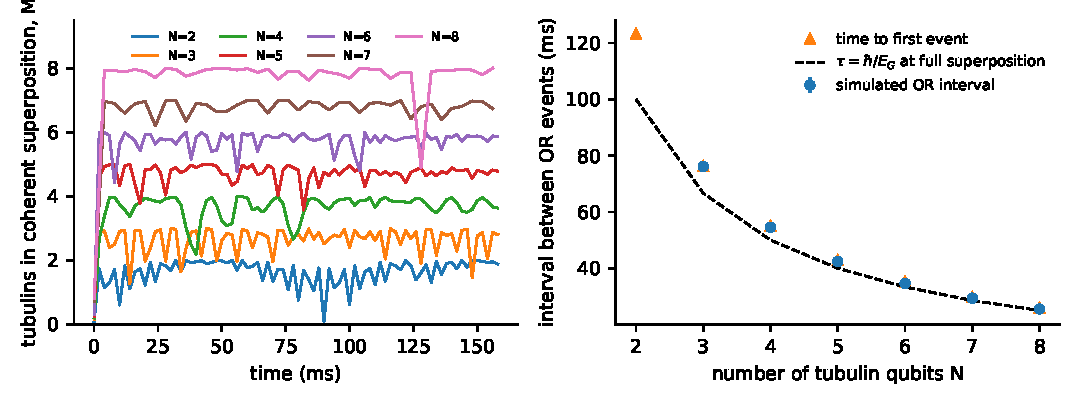
\includegraphics[width=\textwidth]{../figures/fig1_scaling.pdf}
\caption{Left: ensemble-mean $M(t)$ for $N=2$--\Nmax\ qubits under the jump rule; each sawtooth drop is an OR event. Right: mean interval between events versus $N$ (points, $\pm$ s.d.) against $\tau=\hbar/E_G$ evaluated at full superposition (dashed).}
\label{fig:scaling}\end{figure}
Figure~\ref{fig:scaling} and Table~\ref{tab:scaling} show the jump dynamics with no environmental decoherence. Coherence builds to $M\approx N$ within a few milliseconds and events recur at intervals that track $\hbar/E_G$ at full superposition, exceeding it by \ExcessMinMs--\ExcessMaxMs~ms because the superposition is not full while it is forming. With $N=\Nmax$ qubits standing for the calibrated $2\times10^{10}$ tubulins the interval is \IntervalNeight~ms against the predicted \PredNeight~ms. This is not a test of the theory, since the calibration was chosen to give 25~ms; it is a check that the implementation respects it, and it establishes the baseline against which decoherence is measured.

\begin{table}[t]\centering\small
\begin{tabular}{ccccc}\toprule
$N$ & $\tau=\hbar/E_G$ (ms) & OR interval (ms) & first event (ms) & max $\langle M\rangle$\\\midrule
\ScalingRows
\bottomrule\end{tabular}
\caption{Jump-rule statistics versus chain length, $\gamma=0$. Each qubit represents $2\times10^{10}/8$ tubulins.}
\label{tab:scaling}\end{table}

\subsection{Moments require a decoherence time of order $\TdecStarMs$~ms}
\begin{figure}[t]\centering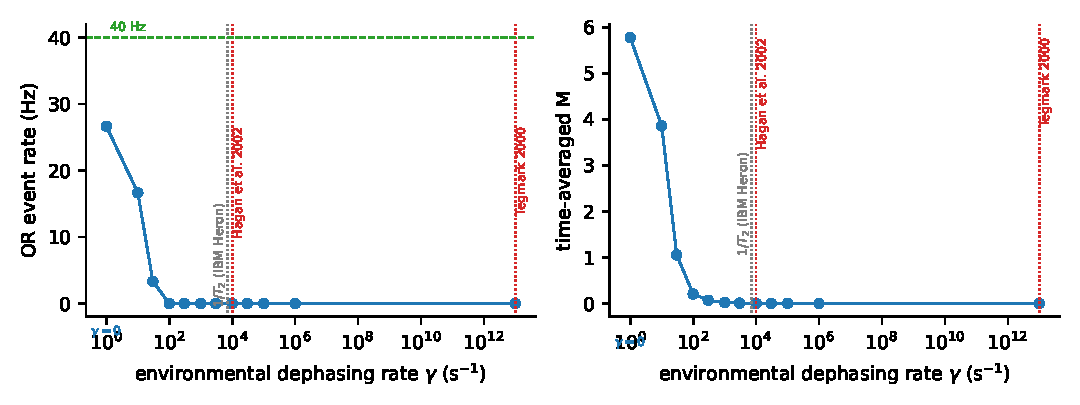
\includegraphics[width=\textwidth]{../figures/fig2_decoherence.pdf}
\caption{$N=6$. Left: OR event rate versus environmental dephasing rate $\gamma$ (leftmost point $\gamma=0$). Right: time-averaged $M$. Dotted lines mark the Hagan et al.\ and Tegmark estimates and the intrinsic dephasing rate $1/T_2$ of the IBM Heron calibration used in Sec.~\ref{sec:circuit}.}
\label{fig:dec}\end{figure}
Figure~\ref{fig:dec} and Table~\ref{tab:dec} sweep $\gamma$ for $N=6$. At $\gamma=0$ the event rate is \RateZero~Hz. The rate halves at $\gamma^\ast\approx\GammaStar$~s$^{-1}$, a decoherence time of about $\TdecStarMs$~ms, and collapses to zero well before the Hagan et al.\ value, where the time-averaged $M$ is $\MHagan$ and the rate is \RateHagan~Hz. At the Tegmark rate $M=\MTegmark$: no superposition ever forms. The reason the threshold is so much longer than 25~ms is that $\int E_G\,dt$ must reach $\hbar$ while coherence is being continuously eroded; the superposition has to be nearly complete for tens of milliseconds, not merely present for an instant. In this model, therefore, the requirement for 40~Hz Orch-OR moments is a microtubule decoherence time about $\GapHagan$ times longer than the most favourable published estimate and $\GapTegmarkOrders$ orders of magnitude longer than Tegmark's.

\begin{table}[t]\centering\small
\begin{tabular}{ccc}\toprule
$\gamma$ (s$^{-1}$) & event rate (Hz) & $\langle M\rangle_t$\\\midrule
\DecoherenceRows
\bottomrule\end{tabular}
\caption{Decoherence sweep, $N=6$, three trajectories of 300~ms each.}
\label{tab:dec}\end{table}

\subsection{The two readings of $\tau=\hbar/E_G$ are not equivalent}
\begin{figure}[t]\centering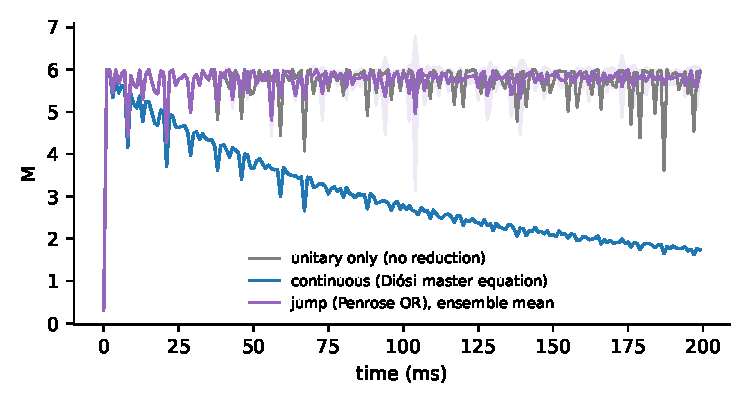
\includegraphics[width=0.75\textwidth]{../figures/fig3_unravelling.pdf}
\caption{$N=6$, $\gamma=0$. $M(t)$ under unitary evolution alone (grey), the continuous Di\'osi rule (blue), and the jump rule averaged over 12 trajectories (purple, band $\pm$ s.d.).}
\label{fig:unr}\end{figure}
Figure~\ref{fig:unr} compares the two implementations at identical $E_G$. The jump rule gives periodic events with mean interval $\JumpInterval\pm\JumpIntervalSd$~ms and a time-averaged $M$ of \JumpMavg. The continuous rule gives no events at all: coherence settles to a steady partially coherent value $\langle M\rangle_t=\ContMavg$ in which the drive and the gravitational dephasing balance. Both are ``$\tau=\hbar/E_G$''. Orch-OR needs the first reading, discrete reductions that can be identified with moments; but the master-equation form is the one that has been tested experimentally \citep{donadi2021}. A simulation makes explicit that these are different physical hypotheses, not two descriptions of one process, and that the ensemble average of the jump dynamics (purple) does not reproduce the continuous dynamics (blue).

\subsection{On a quantum circuit under hardware noise}\label{sec:circuit}
\begin{figure}[t]\centering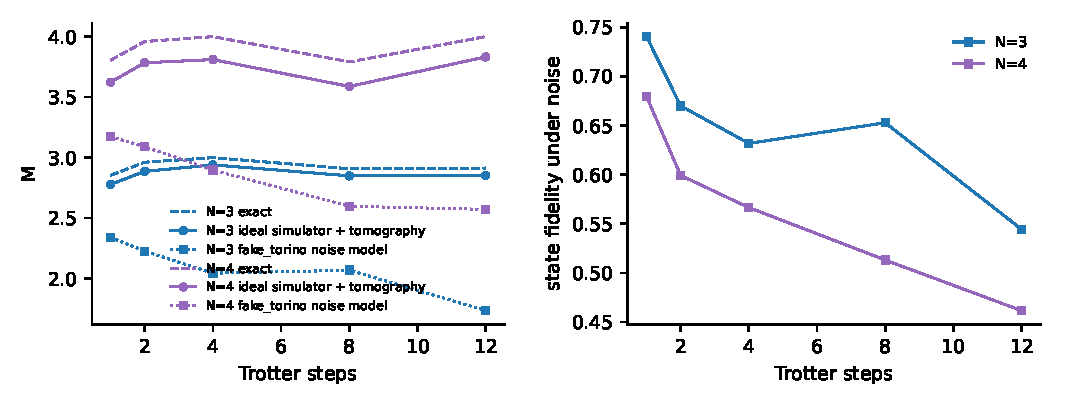
\includegraphics[width=\textwidth]{../figures/fig4_circuit.pdf}
\caption{Trotterised circuit, $N=3,4$. Left: $M$ from the exact state (dashed), from tomography on the ideal simulator (circles), and from tomography under the \Backend\ noise model (squares). Right: fidelity of the noisy state to the exact one.}
\label{fig:circ}\end{figure}
Figure~\ref{fig:circ} and Table~\ref{tab:circ} show the same model as a circuit. Tomography on the ideal simulator recovers $M$ to within sampling error. Under the calibrated noise model, coherence is lost steadily with circuit depth: after \StepsLast\ Trotter steps on four qubits, $M$ falls from $\MexactNfourLast$ (exact) to $\MnoisyNfourLast$ and the state fidelity to $\FidelityNfourLast$. The device's intrinsic dephasing rate, $1/T_2\approx\GammaHW$~s$^{-1}$, is of the same order as the Hagan et al.\ estimate for microtubules and about $\GammaHWoverStar$ times the threshold $\gamma^\ast$ found above. Two conclusions follow. First, a present-day superconducting processor is, for this purpose, roughly as noisy as the most optimistic model of a microtubule, so running Orch-OR dynamics on hardware is a decoherence experiment of the same kind the theory faces in the brain. Second, the observable that the theory cares about, $M$, is not directly measurable: it required full tomography, $3^N$ circuits, which is the reason we stop at $N=4$ and the reason any hardware test of this kind will be limited to a handful of tubulin qubits.

\begin{table}[t]\centering\small
\begin{tabular}{cccccccc}\toprule
$N$ & steps & sim.\ time (ms) & 2q gates & $M$ exact & $M$ ideal tomo & $M$ noisy tomo & fidelity\\\midrule
\CircuitRows
\bottomrule\end{tabular}
\caption{Circuit study on Qiskit Aer with the \Backend\ noise model; 2000 shots per tomography basis.}
\label{tab:circ}\end{table}

\section{Discussion}
What the simulation adds to the order-of-magnitude debate is a quantitative statement that depends on the theory's own calibration and on nothing else: a periodic 40~Hz sequence of reductions requires sustained coherence for of order $\TdecStarMs$~ms, not 25~ms, because the action must integrate to $\hbar$ while the superposition is still forming and while anything that dephases it is acting. Whether a biological system can achieve that is the open empirical question; the simulation does not answer it, but it sharpens what ``shielding'' would have to deliver. The second point is that the jump and master-equation forms of DP collapse, which are often treated as interchangeable, give different observable dynamics here, and only one of them produces anything that could be called a moment. The third is practical: hardware simulations of Orch-OR are possible today for a few qubits, but they inherit a decoherence rate comparable to the Hagan et al.\ estimate, so what they test is the robustness of the dynamics to noise rather than gravity.

\section{Limitations}
The Hamiltonian is a generic transverse-field Ising chain, not a model of tubulin electrostatics; the coupling and drive were chosen to produce millisecond-scale coherence growth. $E_G$ is linear in $M$, following the Hameroff--Penrose estimate, and ignores spatial structure. No gravitational physics is simulated; DP enters only through the rate $\epsilon_q/\hbar$ and the threshold rule. The jump rule is one of several ways to make Penrose's lifetime statement precise. The representation scale $10^x$ is a device for connecting a few qubits to $10^{10}$ tubulins and should not be over-read. The circuit study used a calibrated noise model of a real device, not the device itself; a hardware run of the $N=3,4$ circuits is straightforward and is left for follow-up. None of these choices affects the qualitative conclusions, but each affects the numbers at the factor-of-a-few level.

\section{Availability}\label{sec:avail}
Code (Python, NumPy/SciPy, Qiskit), raw results, figures, the macro file and this manuscript are at \url{https://github.com/wonmor/orch-or-quantum} under the MIT licence. The classical interactive model is at \url{https://github.com/wonmor/OrchOR} with a browser version at \url{https://wonmor.github.io/orch-or/}.

\section*{Author statement}
This work was conceived, designed and carried out by the author alone, without academic supervision, collaborators or institutional support. AI-assisted software tools were used in preparing the code and manuscript. The author takes full responsibility for all content and claims.

\begin{thebibliography}{99}
\bibitem[Di\'osi(1989)]{diosi1989} L.~Di\'osi. Models for universal reduction of macroscopic quantum fluctuations. \emph{Phys. Rev. A} 40, 1165 (1989).
\bibitem[Donadi et al.(2021)]{donadi2021} S.~Donadi, K.~Piscicchia, C.~Curceanu, L.~Di\'osi, M.~Laubenstein, A.~Bassi. Underground test of gravity-related wave function collapse. \emph{Nature Physics} 17, 74 (2021).
\bibitem[Hagan et al.(2002)]{hagan2002} S.~Hagan, S.~R. Hameroff, J.~A. Tuszy\'nski. Quantum computation in brain microtubules: Decoherence and biological feasibility. \emph{Phys. Rev. E} 65, 061901 (2002).
\bibitem[Hameroff and Penrose(1996)]{hameroff1996} S.~Hameroff, R.~Penrose. Orchestrated reduction of quantum coherence in brain microtubules: A model for consciousness. \emph{Mathematics and Computers in Simulation} 40, 453 (1996).
\bibitem[Hameroff and Penrose(2014)]{hameroff2014} S.~Hameroff, R.~Penrose. Consciousness in the universe: A review of the `Orch OR' theory. \emph{Physics of Life Reviews} 11, 39 (2014).
\bibitem[Penrose(1994)]{penrose1994} R.~Penrose. \emph{Shadows of the Mind}. Oxford University Press (1994).
\bibitem[Penrose(1996)]{penrose1996} R.~Penrose. On gravity's role in quantum state reduction. \emph{General Relativity and Gravitation} 28, 581 (1996).
\bibitem[Seong(2026)]{seong2026viz} W.~Seong. Orch-OR Visualizer: an interactive, calibrated model of orchestrated objective reduction for teaching and critique. Zenodo (2026). \url{https://github.com/wonmor/OrchOR}
\bibitem[Tegmark(2000)]{tegmark2000} M.~Tegmark. Importance of quantum decoherence in brain processes. \emph{Phys. Rev. E} 61, 4194 (2000).
\end{thebibliography}
\end{document}
